

{\setbeamercolor{background canvas}{bg=black}
	\begin{frame}[plain]
	
	\vfill
	\Huge\color{white}
	\begin{center}
		\begin{columns}
			\column{.5\textwidth}
			\vspace{7em}
			
			\hfill 
			Earth Observation Data
			\column{.5\textwidth}
			
			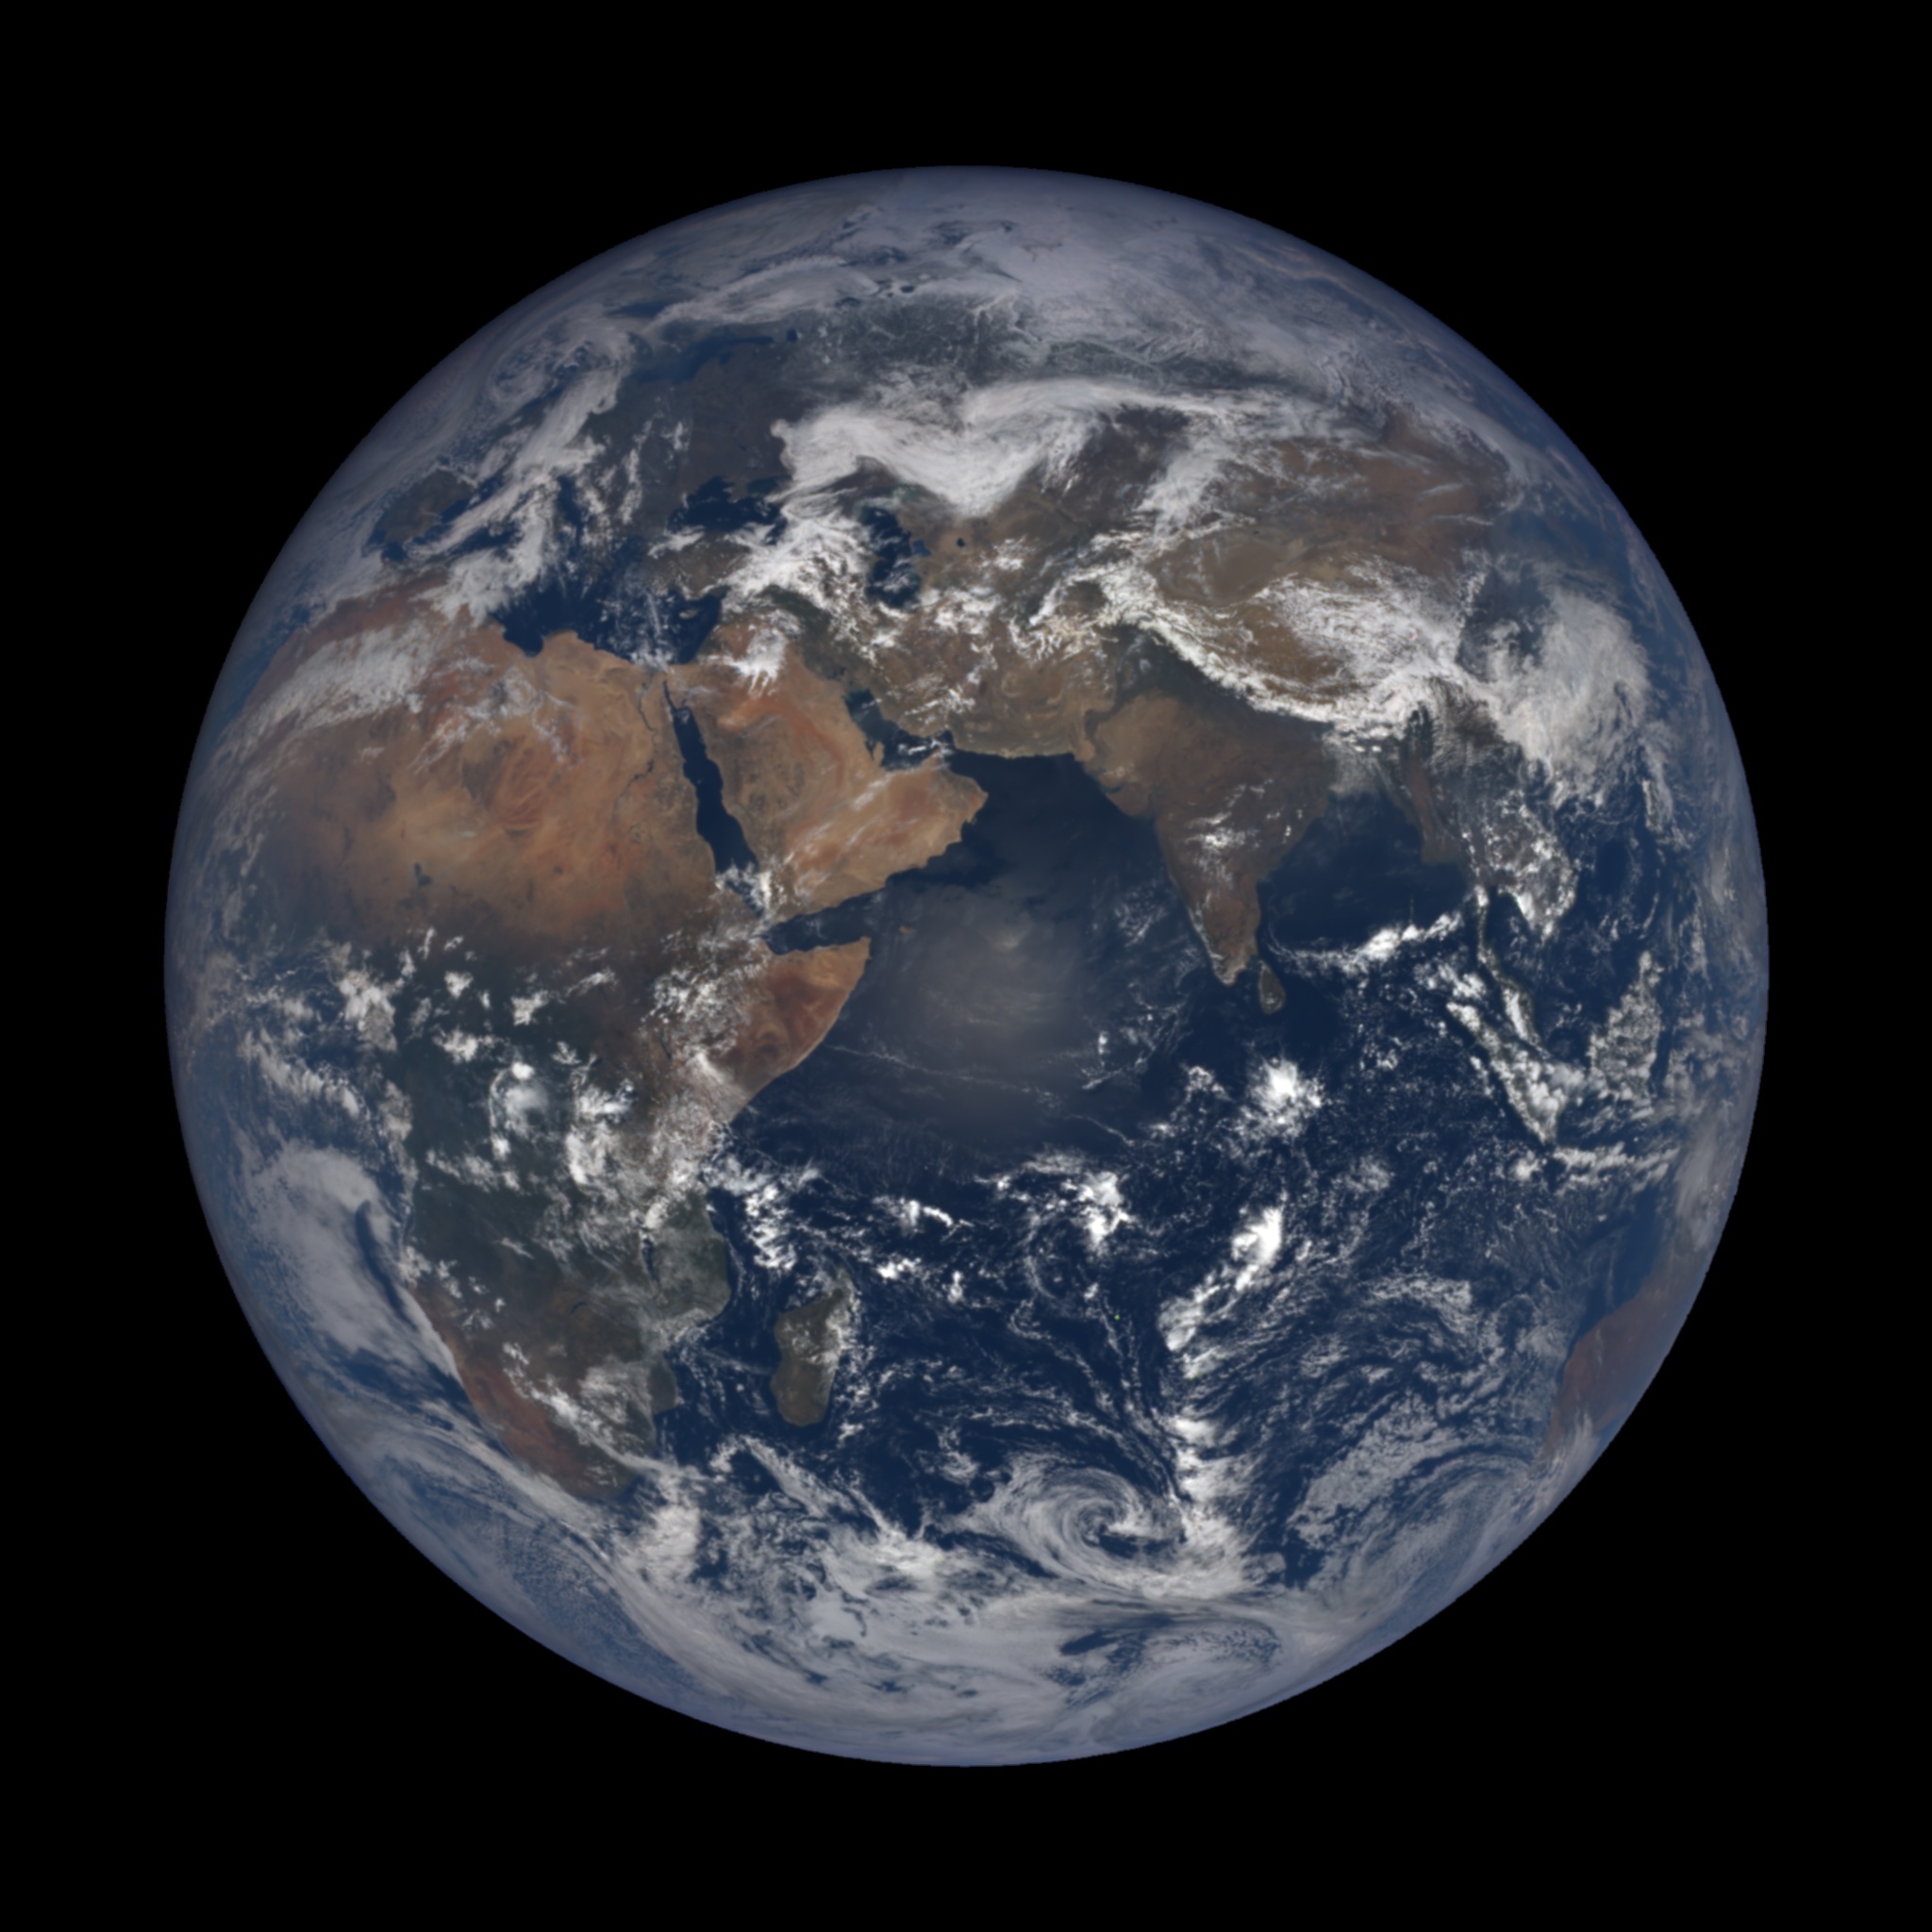
\includegraphics[width=5cm]{images/epic1}
			%\includegraphics[width=7cm]{images/fdl}
		\end{columns}
	\end{center}
	
	\vfill
\end{frame}
}

\begin{frame}
\frametitle{System Earth}

\begin{columns}
	
	\column{.5\textwidth}
	
	{
		%		The Earth is a complex system.
		%		Only some components is observable by 
		%		\begin{itemize}
		%			\item satellite-based or
		%			\item in-situ observations
		%		\end{itemize}
		%		
		
		%	\begin{equation*}\V{y} = f({\M{X}})\end{equation*}
		%	partially observe the complex system Earth
		\textbf{Partially measuring} System Earth
		{\Huge
			\begin{equation*}
			\M{X} = \sat\left({\earth}\right)
			\end{equation*}
		}
		
		\vspace{1em}
		\textbf{knowledge extraction} through pattern recognition and machine learning
		
		{\Huge\begin{equation*}\V{?} = f({\M{X}})\end{equation*}}
	}
	
	\column{.5\textwidth}
	
	\begin{tikzpicture}[xscale=3, yscale=2]
	\node(earth) at (0,0) {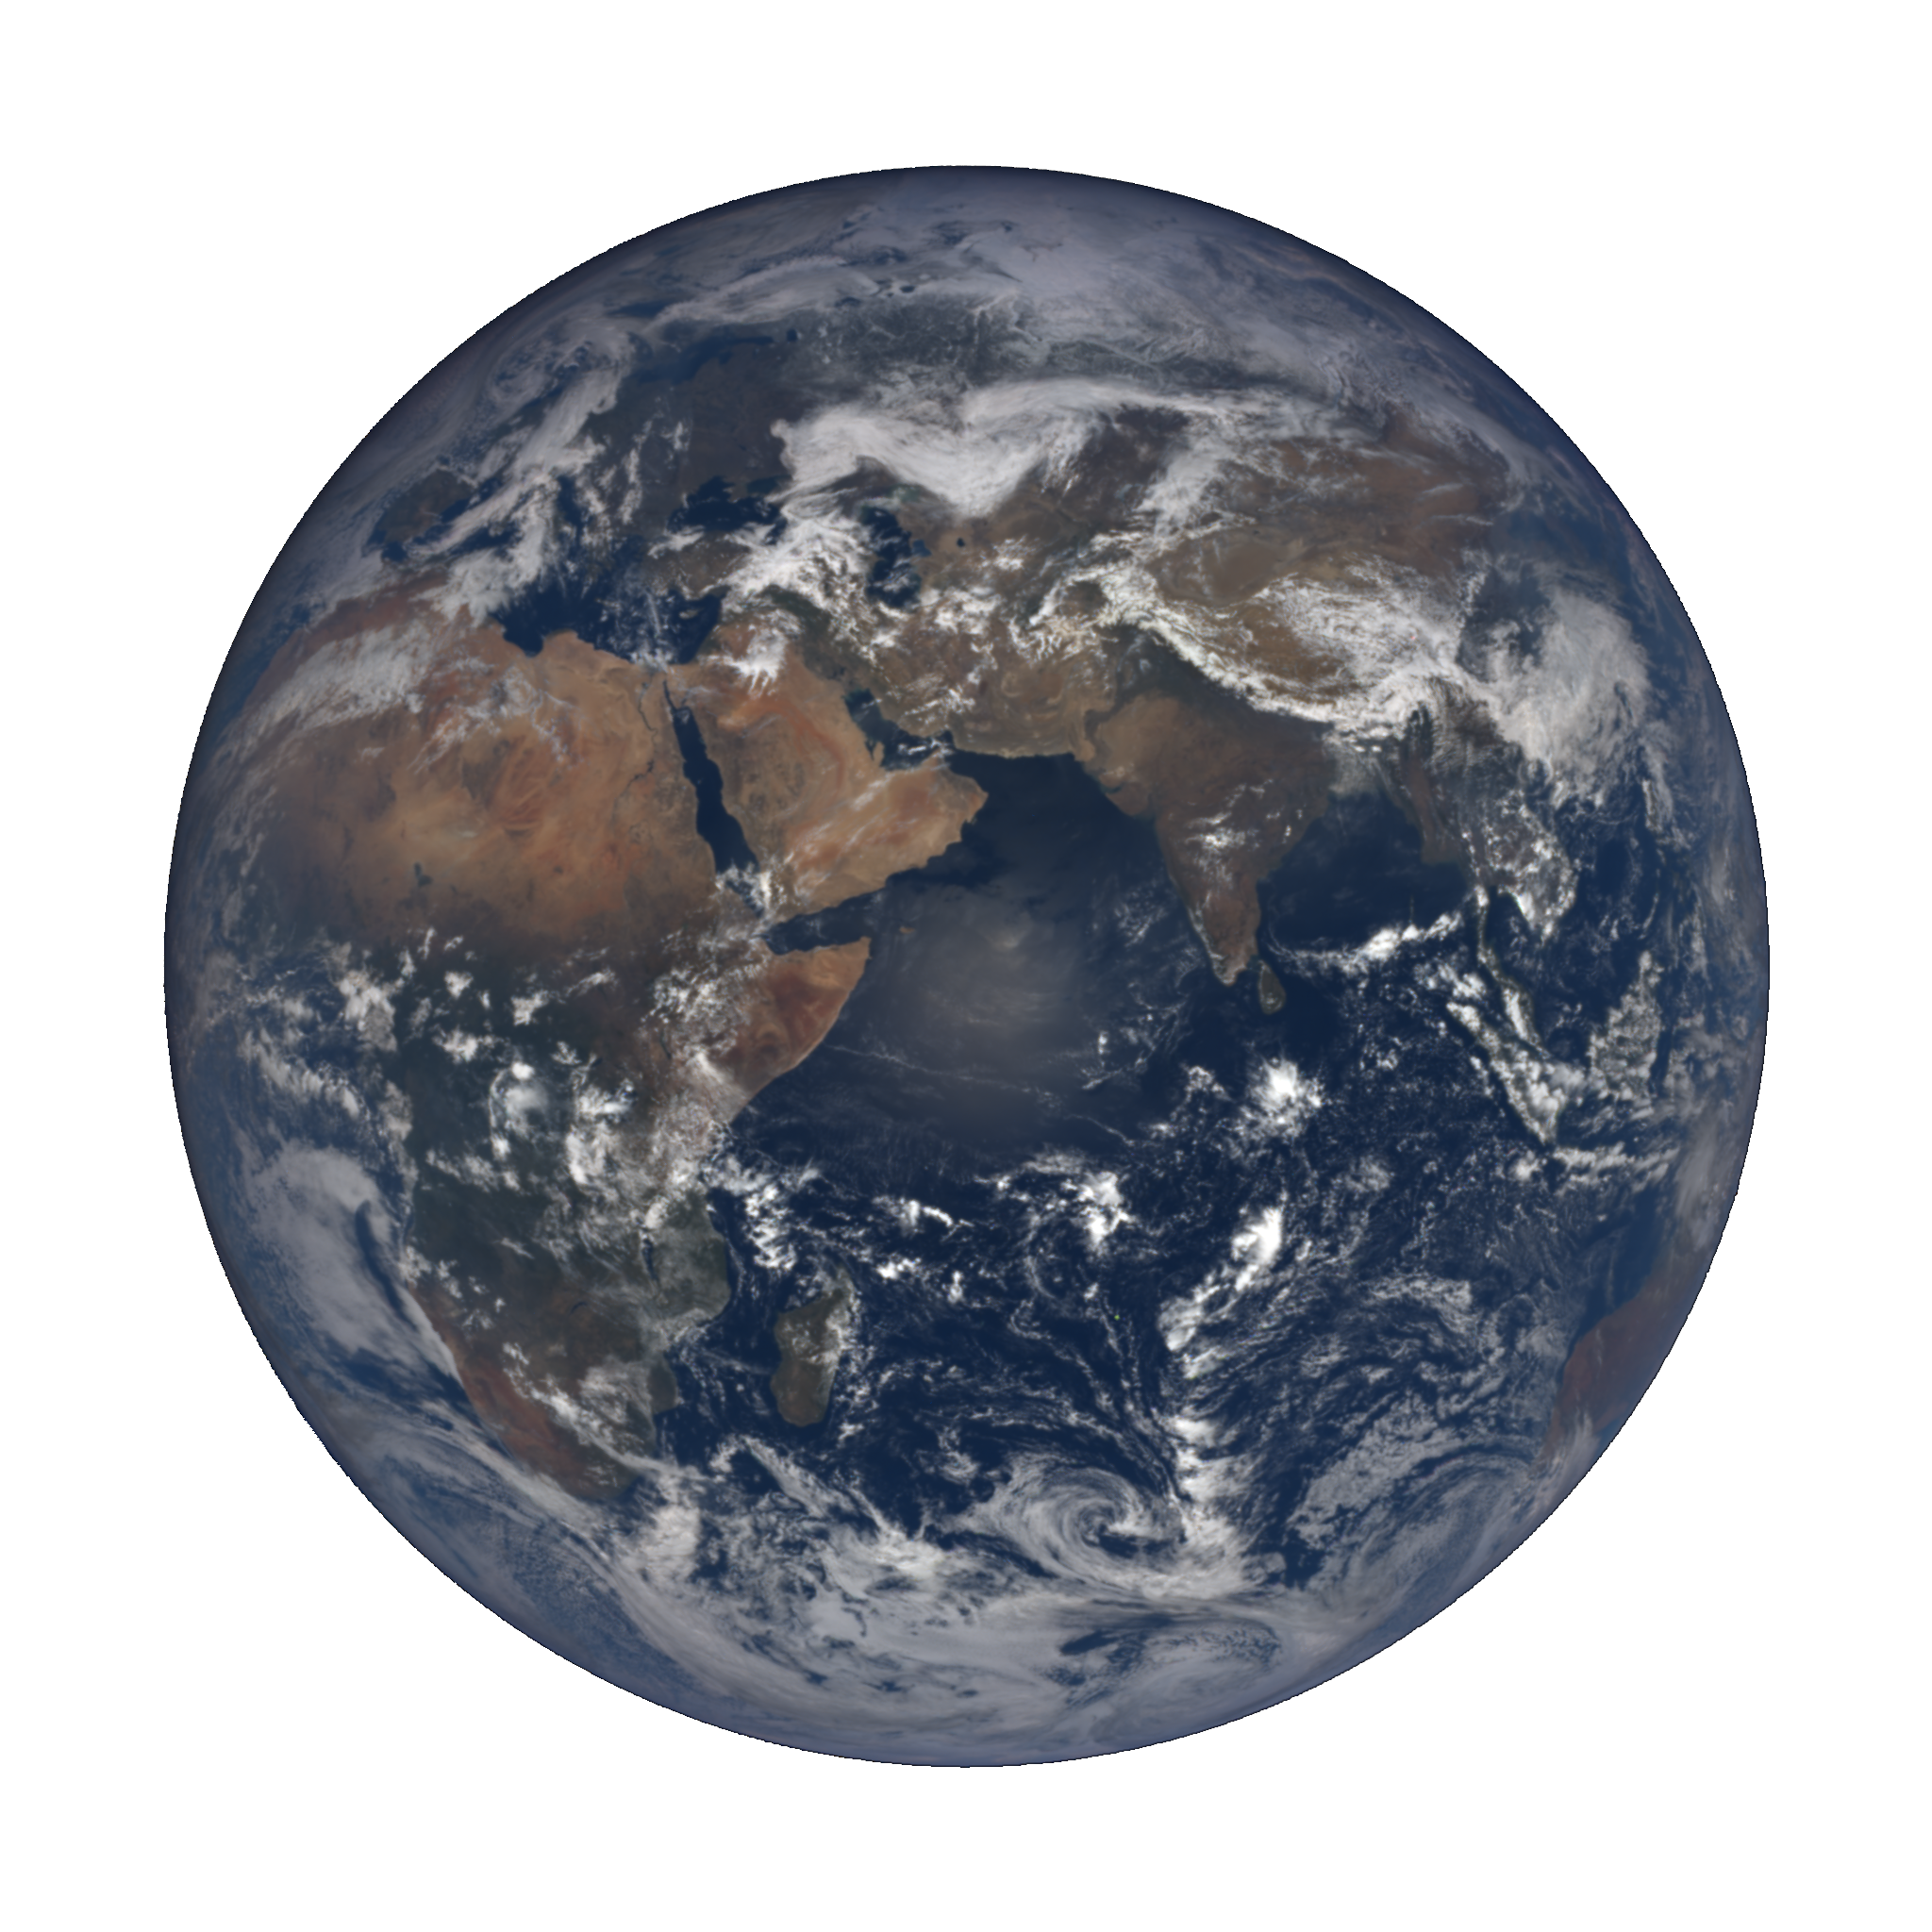
\includegraphics[width=7cm]{images/epicw1}};	
	
	\end{tikzpicture}
	
	
\end{columns}

%	\includegraphics[width=5cm]{images/Earth_gravity}
%	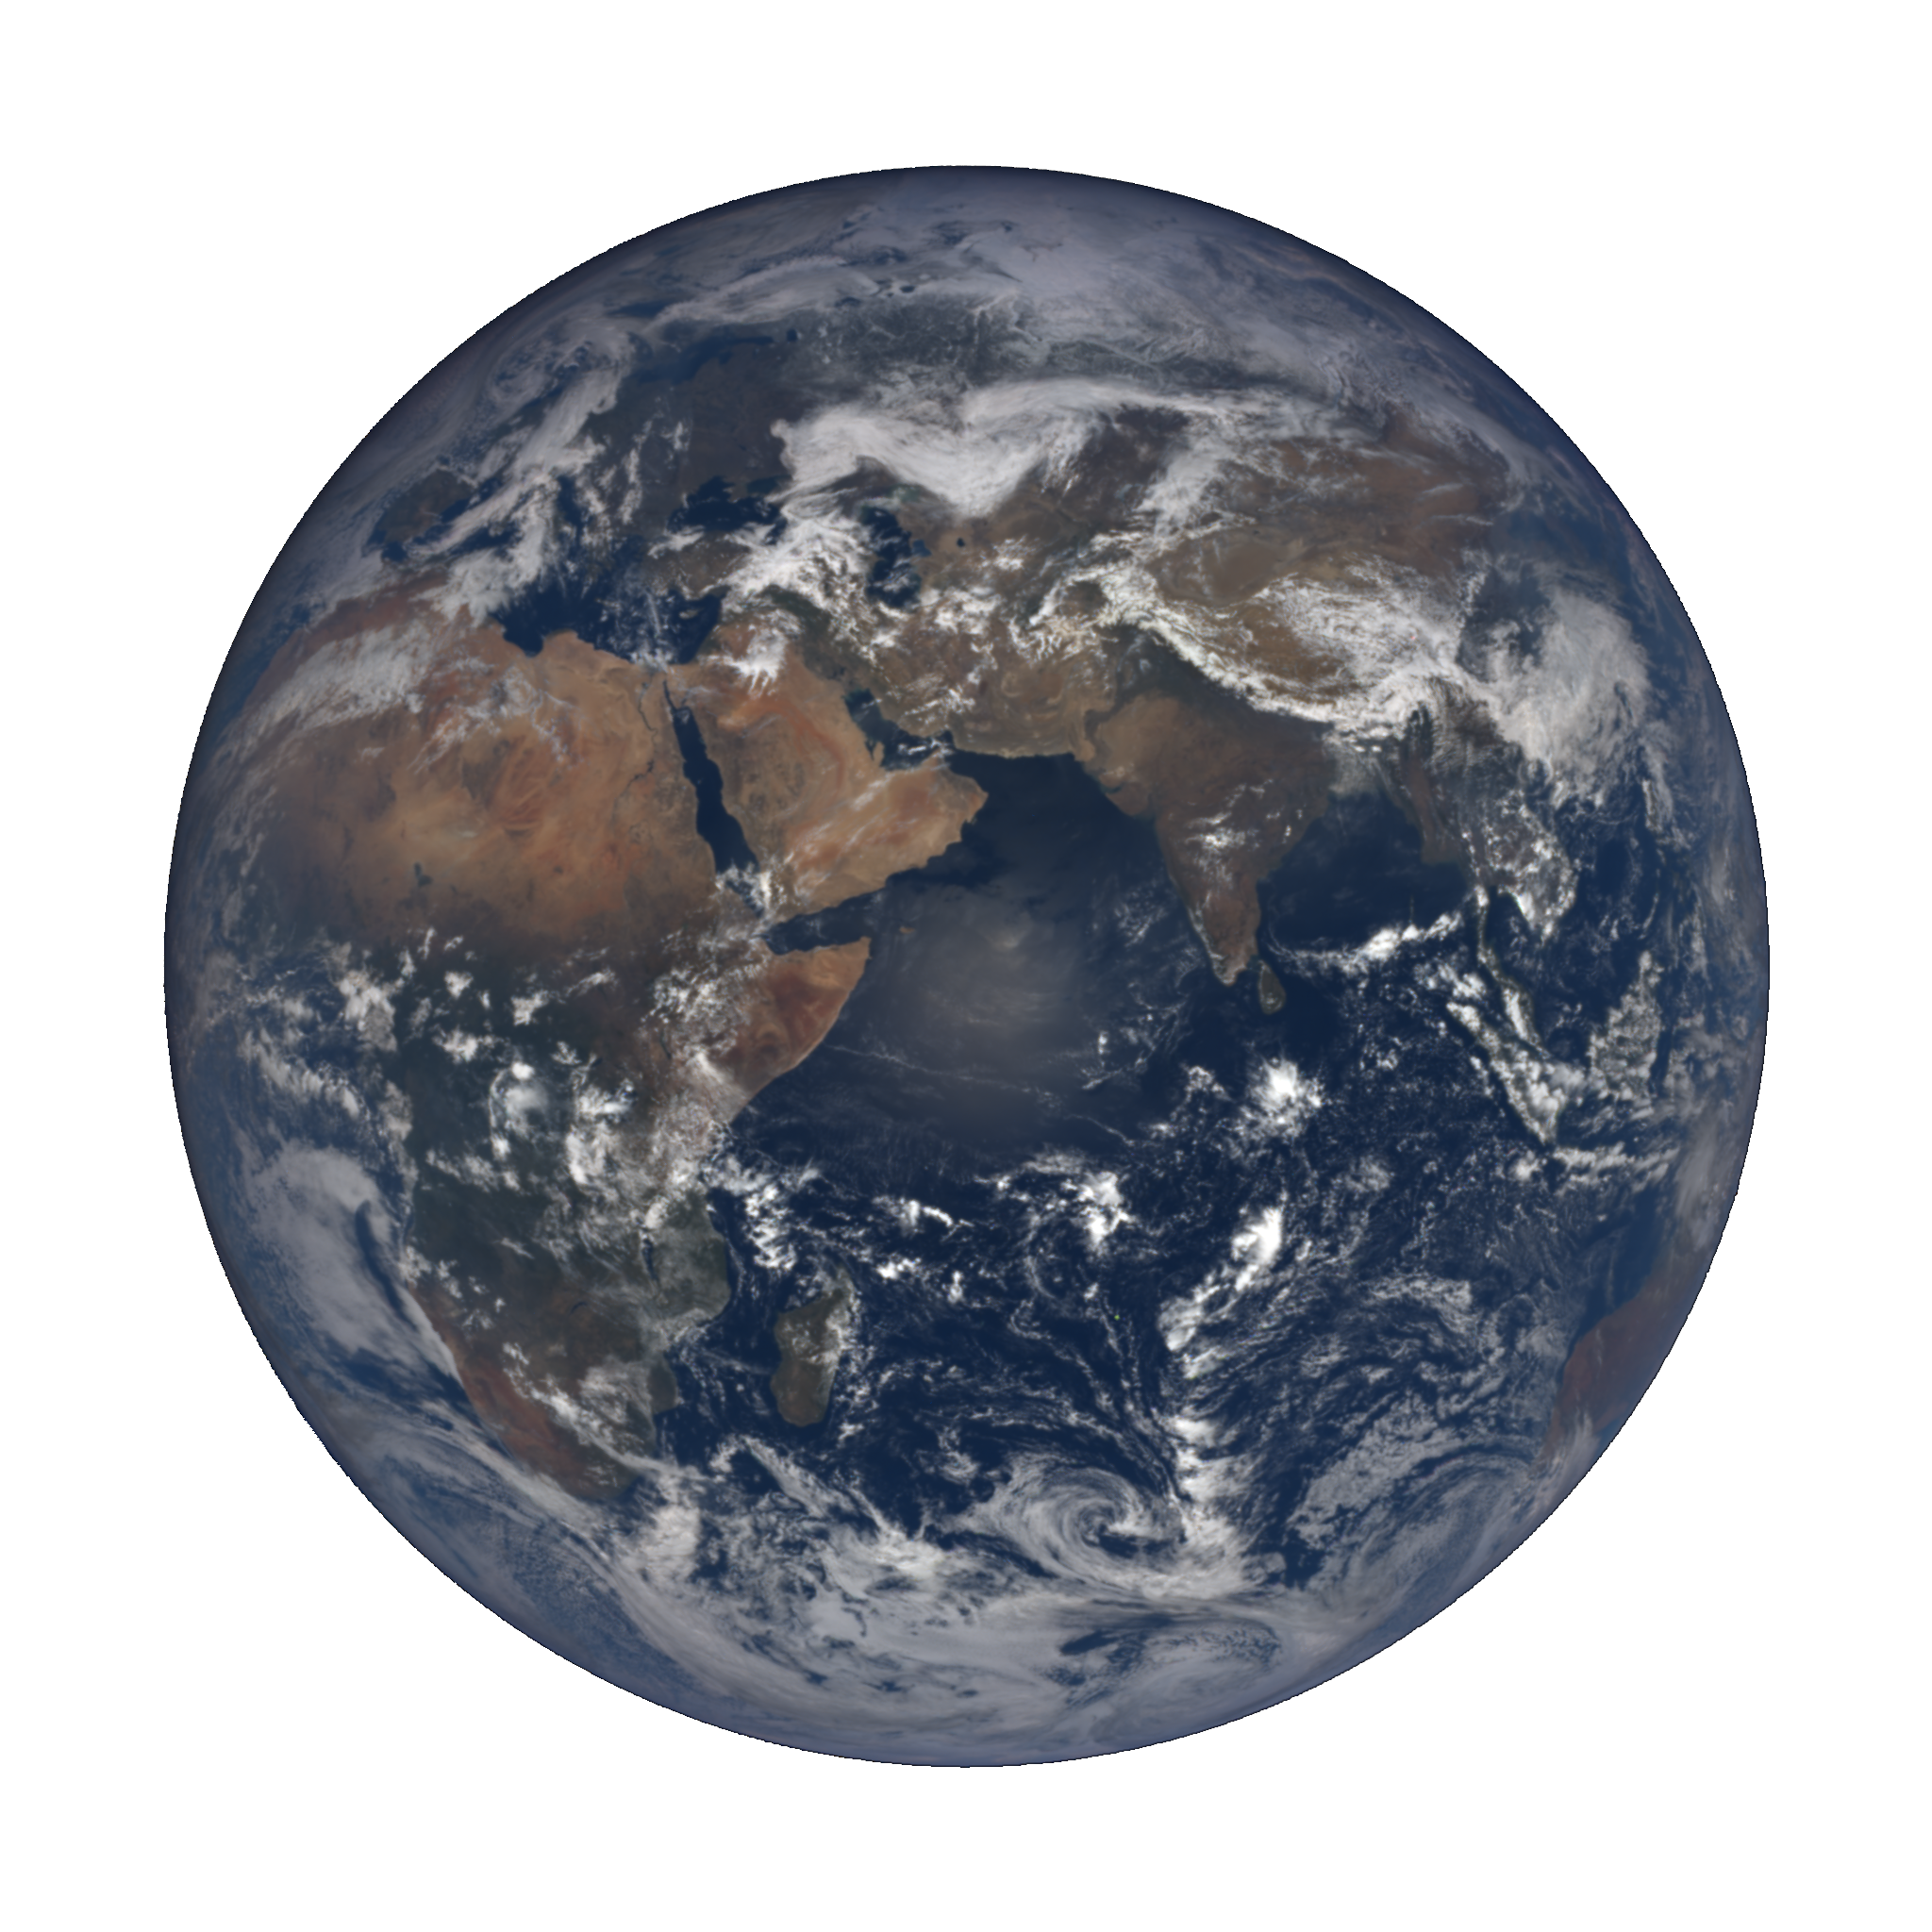
\includegraphics[width=5cm]{images/epicw1}
%	\includegraphics[width=5cm]{images/earthnullschool/sealevelpressure}
%	\includegraphics[width=5cm]{images/earthnullschool/misery_index}
%	\includegraphics[width=5cm]{images/earthnullschool/temp}
%	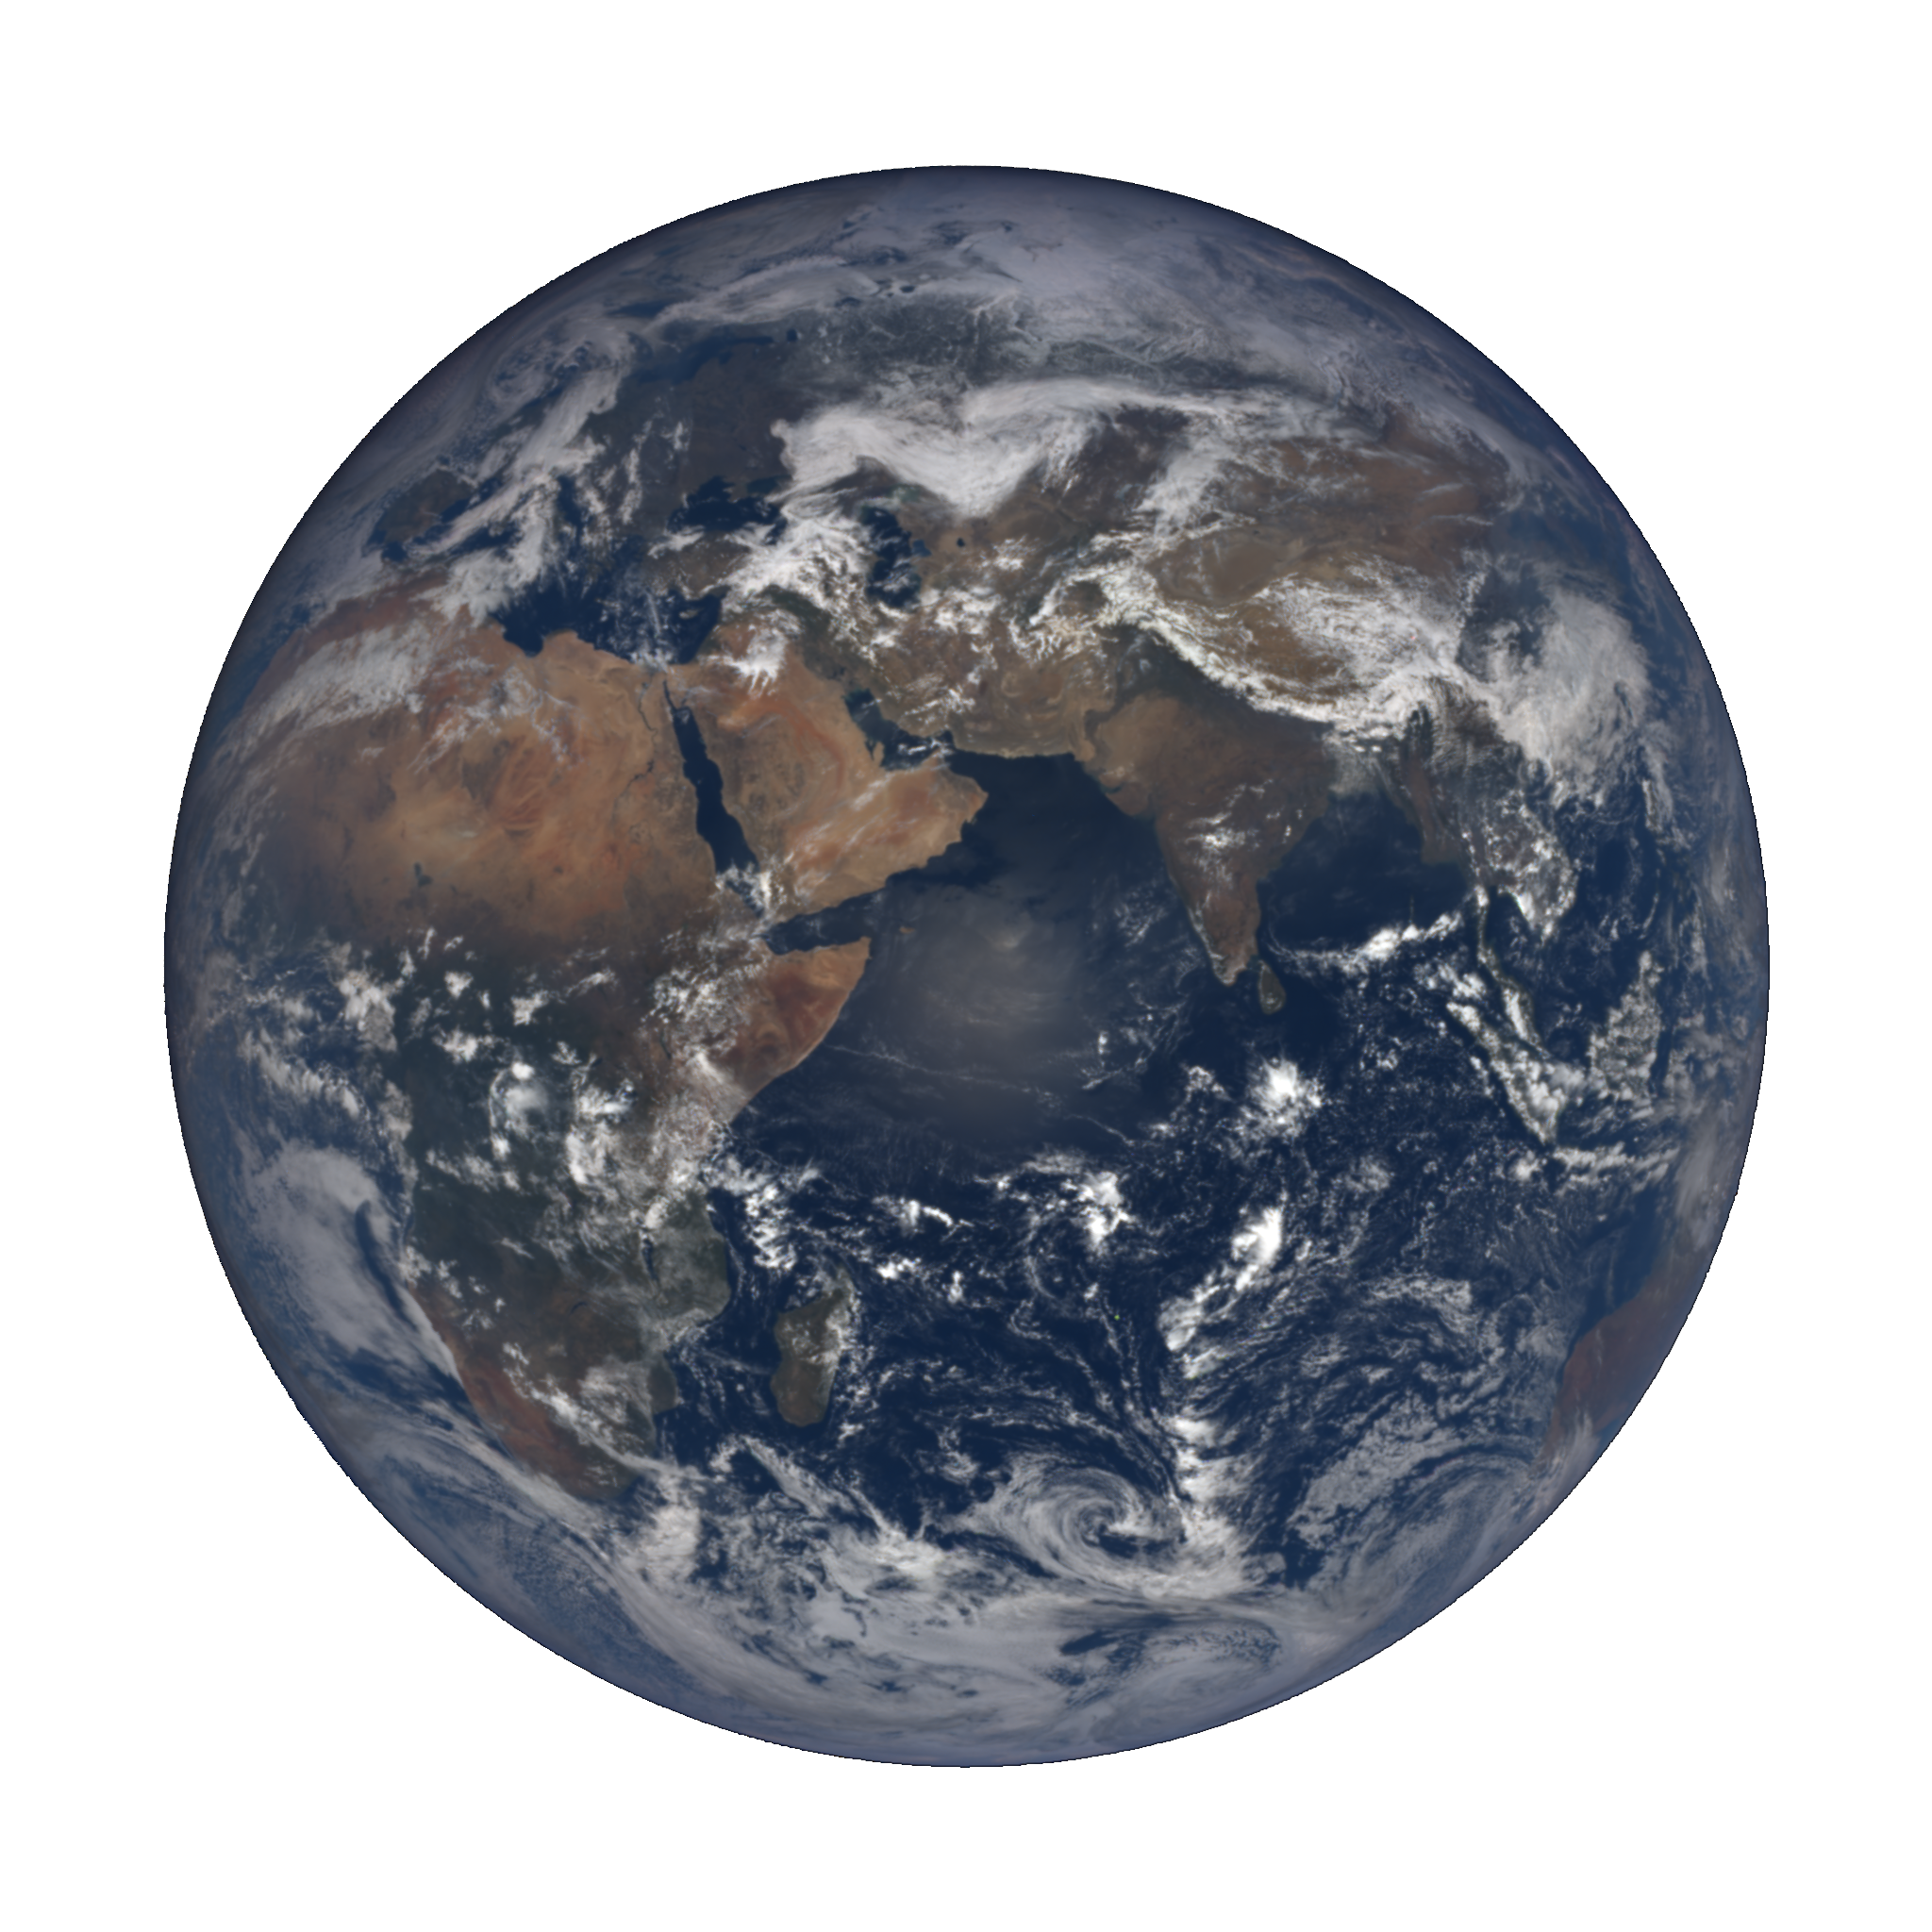
\includegraphics[width=5cm]{images/epicw1}
\end{frame}

%\begin{frame}
%\frametitle{Optical Satellites}
%\begin{columns}
%	\column{.5\textwidth}
%	
%%	
%%	\begin{itemize}[itemsep=.5em]
%%		\item<1-> Sensor measures \textbf{Digital Numbers} $\text{DN}(\lambda)$ for each wavelength $\lambda$. 
%%		\item<2-> \textbf{Digital Numbers} are normalized to \textbf{Radiance} 
%%		$L(\lambda), \left[\frac{W}{\text{sr}m^2}\right]$ by gain and offset calibration.
%%		\item<3-> Radiance is normalized to \textbf{top-of-atmosphere reflectance} $\rho(\lambda)$
%%		%		\item<4-> \textbf{Bottom-of-atmosphere reflectances} are reconstructed using a functional model of the atmosphere.
%%	\end{itemize}
%%	
%	%	Radiance $R_\lambda$ from measured Digital Numbers via calibrated gain $\alpha$ and offset $\beta$
%	%	\begin{equation*}
%	%		L_\lambda = \alpha \text{DN}_\lambda + \beta, \left[\frac{W}{\text{sr}m^1}\right]
%	%	\end{equation*}
%	%	
%	%	top-of-atmosphere reflectance $\rho_\lambda$ as normalized Radiance $R_\lambda$ with solar 
%	%	\begin{equation*}
%	%	\rho_\lambda = \frac{L_\lambda}{\cos(\varphi_\text{sun})}
%	%	\frac{
%	%		\pi d^2
%	%	}
%	%	{
%	%		E_\text{sun}(\lambda)
%	%	}
%	%	\end{equation*}
%	%	
%	%	\vspace{1em}
%	%	
%	%	\begin{itemize}
%	%		\item measured radiance $L(\lambda)$
%	%		\item solar irradiance $E_\text{sun}(\lambda)$
%	%		\item solar zenith angle $\varphi_\text{sun}$
%	%		\item squared Earth-Sun distance $d$ in AU
%	%	\end{itemize}
%	
%	
%	\column{.5\textwidth}
%	
%	
%	\begin{tikzpicture}
%	
%	
%	%	\draw [black,dotted, fill=tumbluelight,domain=110:70] plot ({13*cos(\x)}, {13*sin(\x)-12.8});
%	\draw [fill=tumivory,domain=110:70] plot ({10*cos(\x)}, {10*sin(\x)-10});
%	%	\draw [fill=tumbluelight,domain=110:70] plot ({12*cos(\x)}f, {12*sin(\x)-10});
%	
%	
%	\node(sun) at (-2,2) {
\includegraphics[width=10mm]{images/icons/sun}};
%	\node[rotate=130,anchor=center](sat) at (2,2) {
\includegraphics[width=10mm]{images/icons/sat2}};
%	
%	\node(px) at ({10*cos(90)}, {10*sin(90)-10.1}){
%		\begin{tikzpicture}[xscale=.5,yscale=.25]
%		\draw[fill=tumbluelight] (0,0) -- (1,0) -- (2,1) -- (1,1) -- (0,0);
%		\end{tikzpicture}
%		%
\includegraphics[width=5mm]{images/icons/house}
%	};
%	
%	\draw[-stealth] (sun) -- node[midway,sloped]{\wave} (px);
%	\draw[-stealth] (px) -- node[midway,sloped]{\wave} (sat);
%	
%	\visible<3->{\draw[-stealth] (sun) -- node[midway,sloped]{\wave} (sat);
%		\draw[draw=tumgray] (px) -- node[at end,left]{$\varphi_\text{sun}$} ++(0,1.4); 
%		\draw [draw=tumgray, domain=130:90] plot ({1*cos(\x)}, {1*sin(\x)});
%	}
%	
%	\node[above=.5em of sun]{$E_\text{sun}(\lambda)$};
%	\visible<1>{\node[above=4em of sat]{$DN(\lambda)$};}
%	\visible<2>{\node[above=4em of sat]{$L(\lambda)$};}
%	\visible<3>{\node[above=4em of sat]{$\rho_\text{toa}(\lambda)$};}
%	%	\visible<4>{\node[above=4em of sat]{$\rho_\text{boa}(\lambda)$};}
%	
%	%		\draw[red] (0,0) sin (1,2);
%	
%\end{tikzpicture}
%\end{columns}
%\end{frame}

\begin{frame}
\frametitle{Acquired in regular time intervals}
\framesubtitle{Sentinel 2 Satellite}

%	\includemovie[
%	poster,
%	text={\small(Loading Circle-m-increase3.mp4)}
%	]{6cm}{6cm}{images/s2orbits.mp4}
%	
%	\movie{loaded}{images/s2orbits.avi}

\begin{columns}
\column{.5\textwidth}

\Large
\begin{itemize}
\item<1-> polar sun-synchronous orbit
\item<2-> single orbit circa 100 minutes
\item<3-> revisit same location after 5 days
\item<4-> acquisition stripe of 290km width
\item<5-> 13 spectral bands
\item<6-> ground resolution 10-60m
\item<7-> global coverage and free of charge
\end{itemize}

\column{.5\textwidth}
%		\only<1>{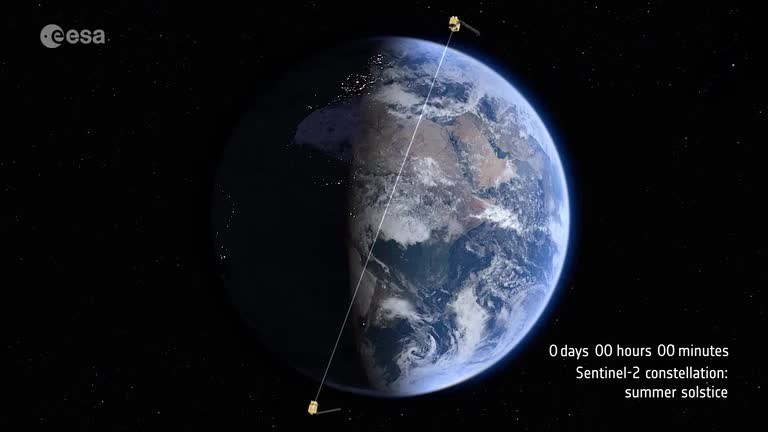
\includegraphics[width=\textwidth]{images/s2orbits/1}}
%		\only<2>{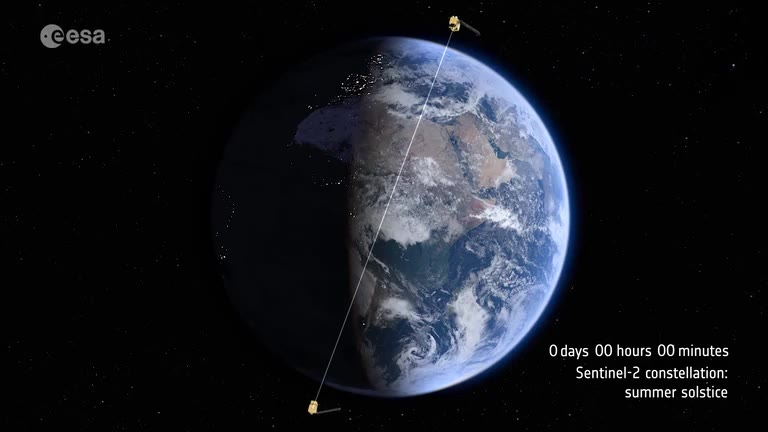
\includegraphics[width=\textwidth]{images/s2orbits/2}}
%		\only<3>{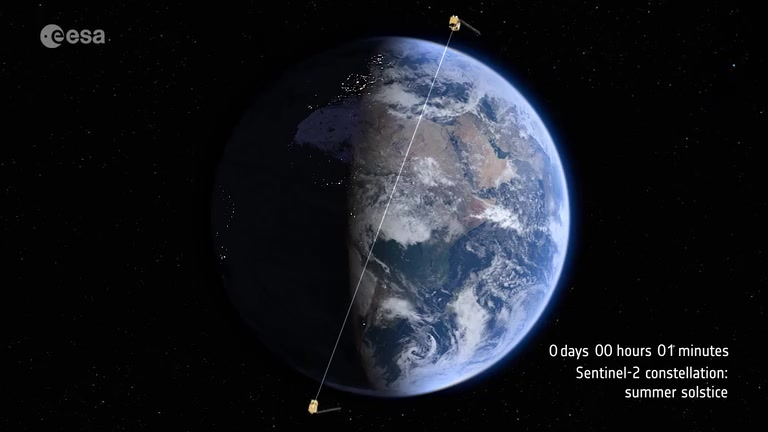
\includegraphics[width=\textwidth]{images/s2orbits/3}}
\only<1>{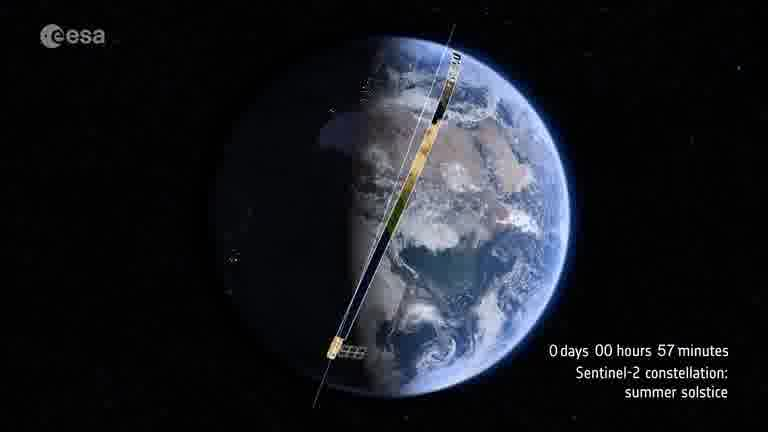
\includegraphics[width=\textwidth]{images/s2orbits/14}}
\only<2>{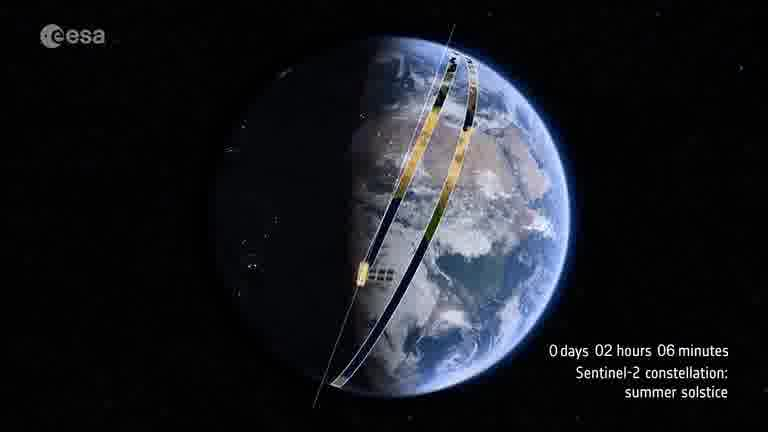
\includegraphics[width=\textwidth]{images/s2orbits/19}}
\only<3>{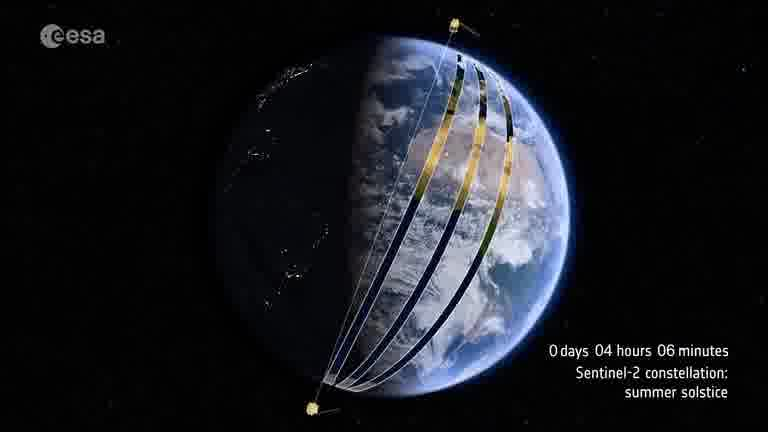
\includegraphics[width=\textwidth]{images/s2orbits/24}}
\only<4>{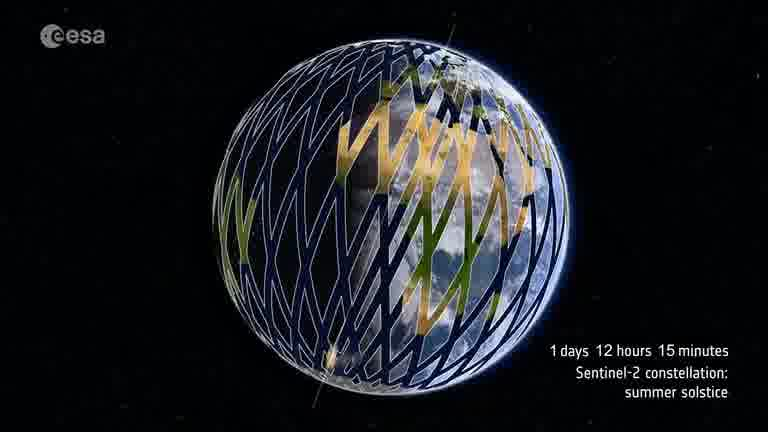
\includegraphics[width=\textwidth]{images/s2orbits/35}}
\only<5>{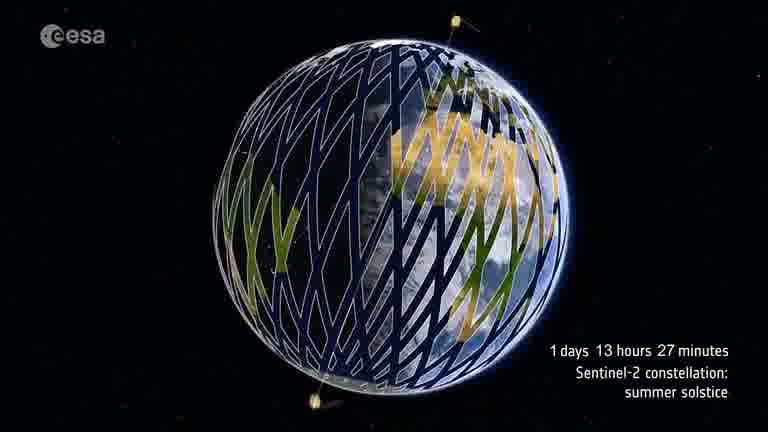
\includegraphics[width=\textwidth]{images/s2orbits/36}}
\only<6>{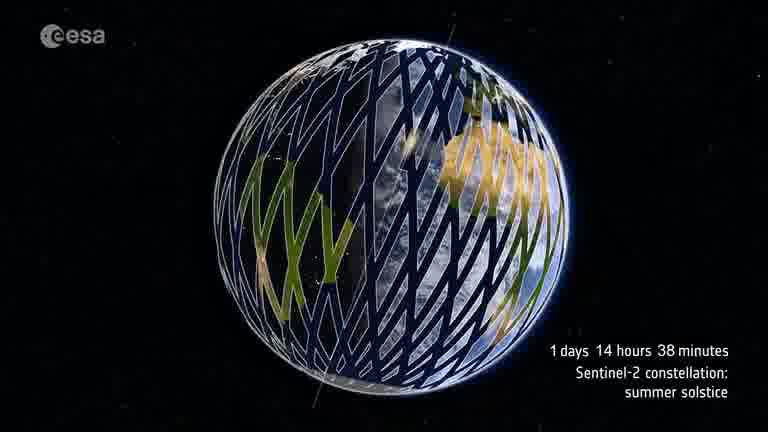
\includegraphics[width=\textwidth]{images/s2orbits/37}}
\only<7>{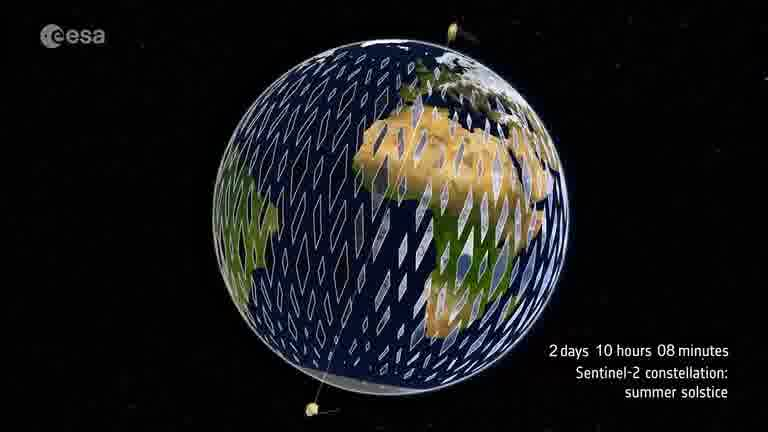
\includegraphics[width=\textwidth]{images/s2orbits/48}}
\tiny\url{https://www.esa.int/spaceinvideos/Videos/2016/08/Sentinel-2_global_coverage}
\end{columns}

\end{frame}

%
%
%{\setbeamercolor{background canvas}{bg=tumblack}
%	\begin{frame}[plain]
%	
%	\vfill
%	\Huge\color{white}
%	\begin{center}
%		\begin{columns}
%			\column{.5\textwidth}
%			\vspace{7em}
%			
%			\hfill 
%			Satellite Data Take-away
%			\column{.5\textwidth}
%			
%			
%			%%			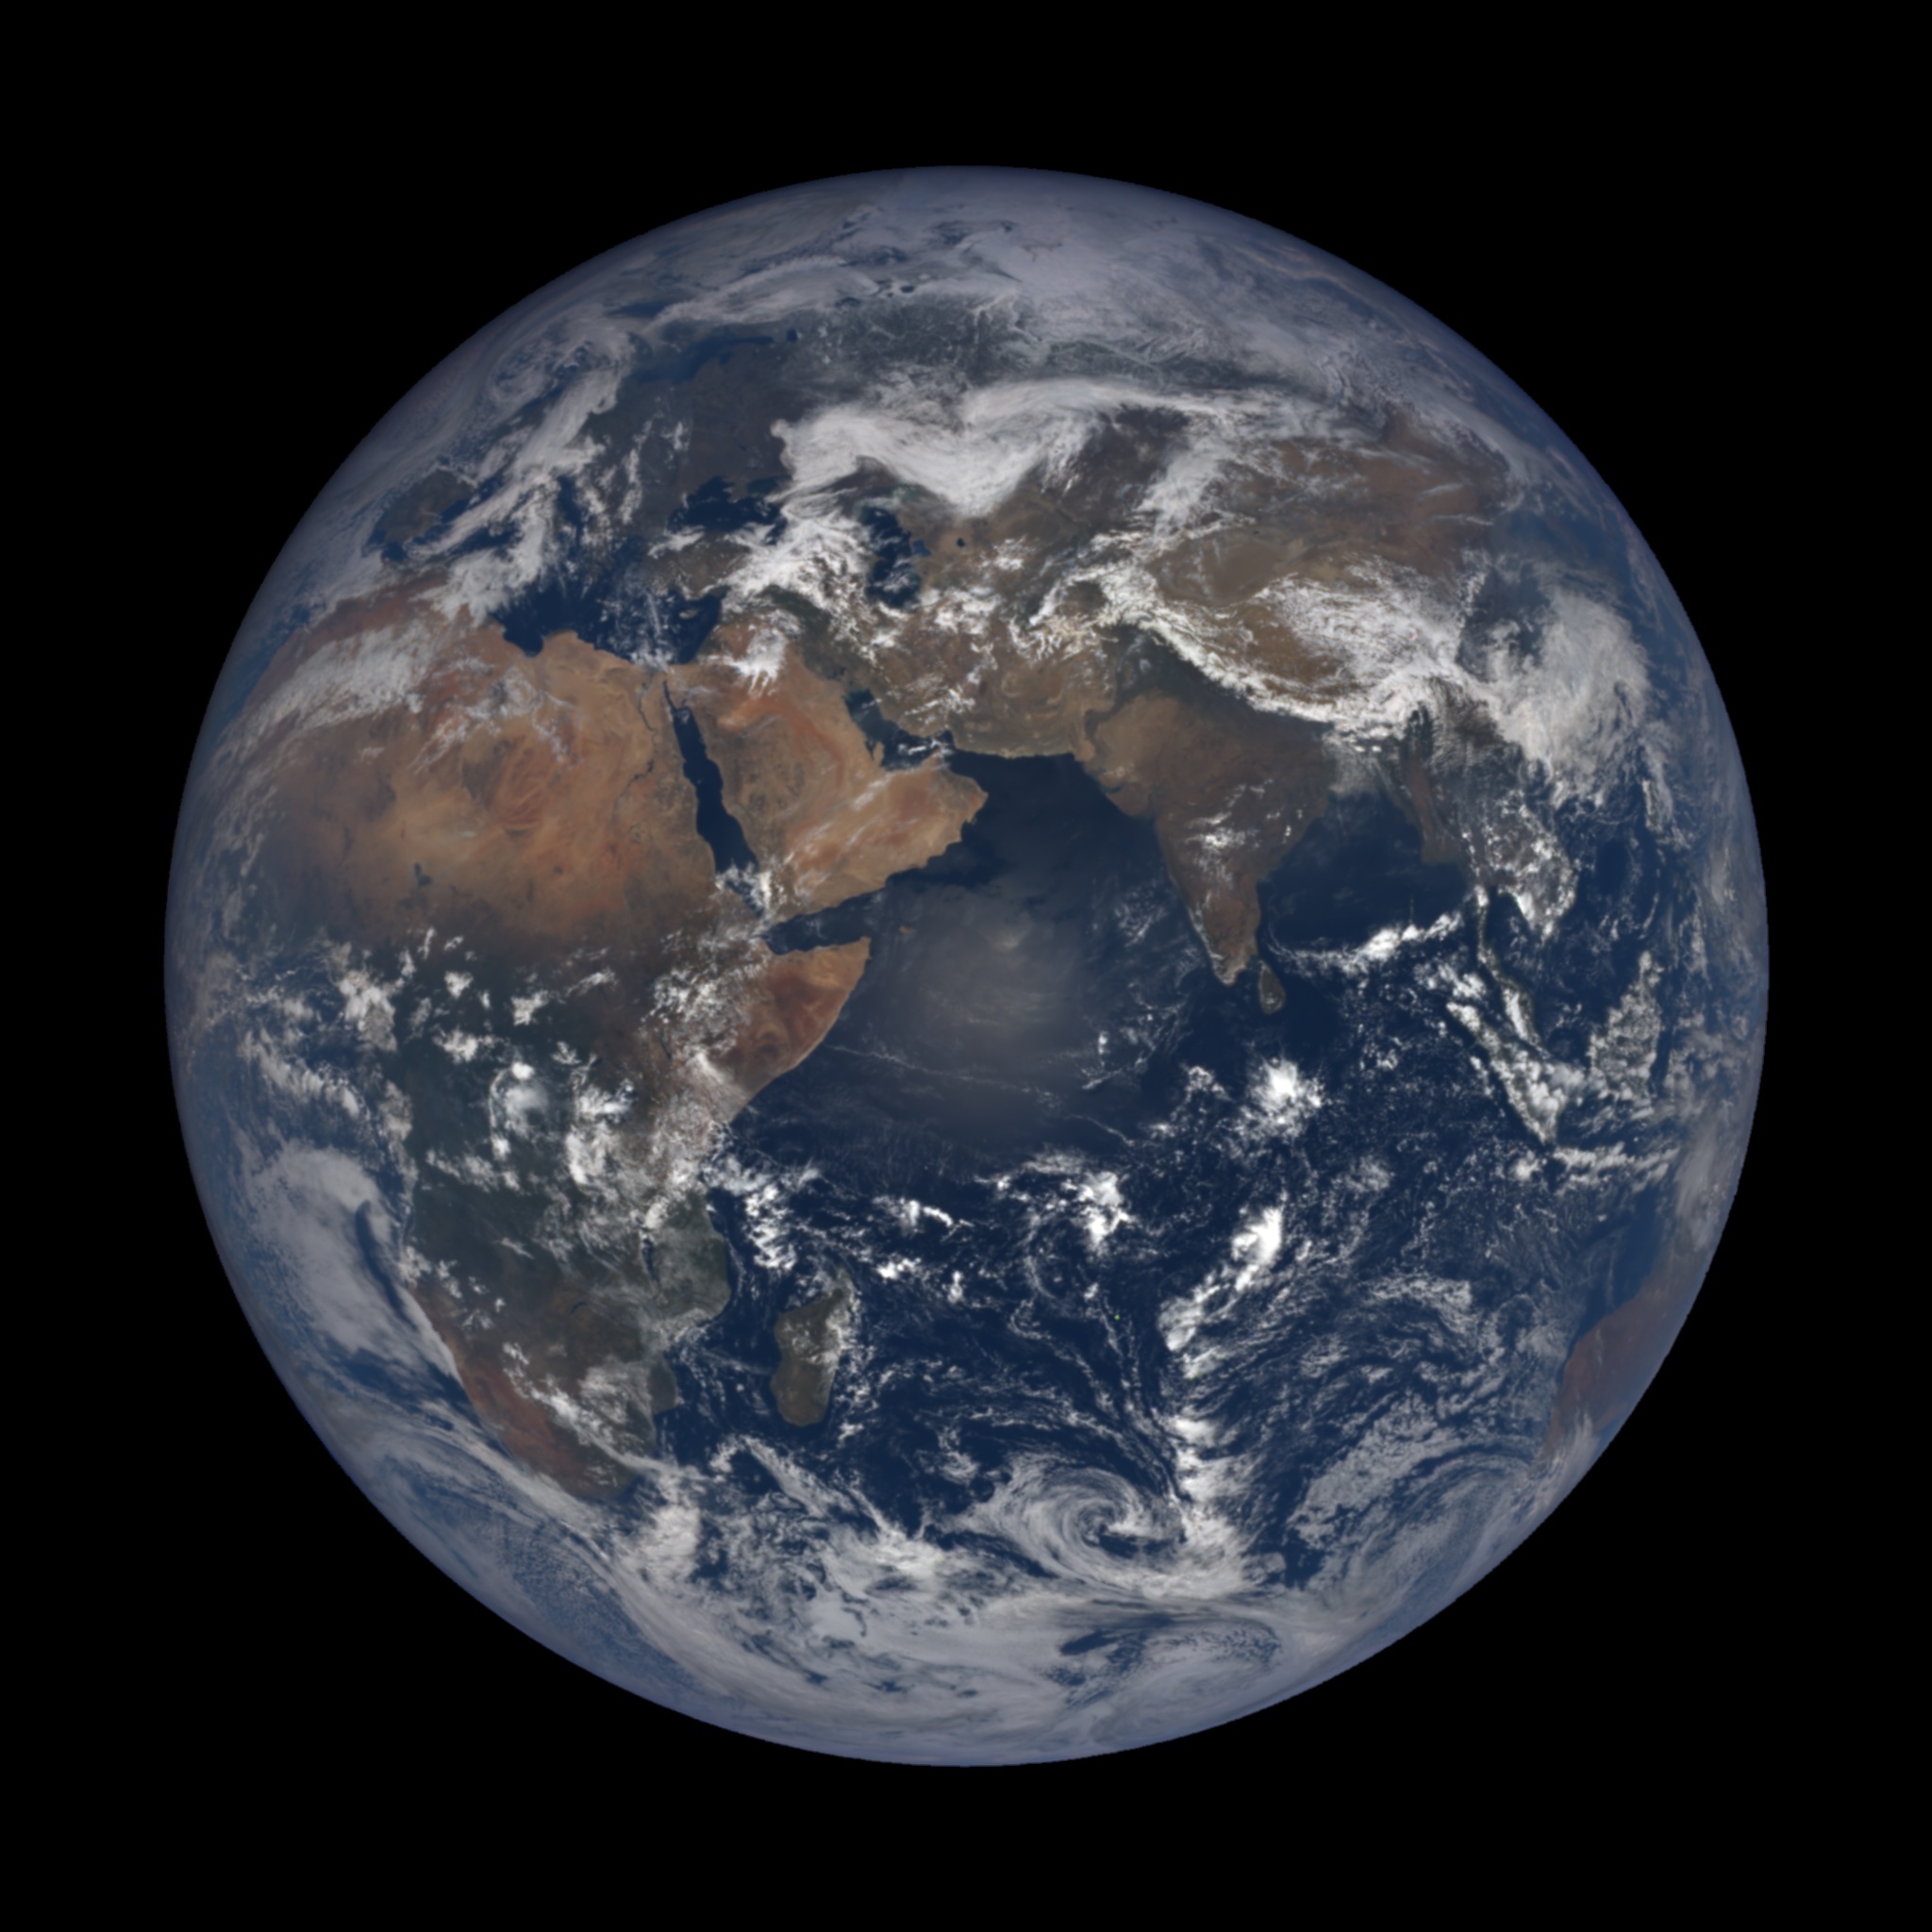
\includegraphics[width=5cm]{images/epic1}
%			%			\includegraphics[width=7cm]{images/fdl}
%		\end{columns}
%	\end{center}
%	
%	\vfill
%\end{frame}
%}

{\setbeamercolor{background canvas}{bg=tumbluedark}
\begin{frame}[plain]

\vfill
\Huge\color{white}
\begin{center}
\begin{columns}
\column{.5\textwidth}
\vspace{7em}

\hfill 
Vegetation Modeling
\column{.5\textwidth}


\includegraphics[width=\textwidth]{images/Large1954_cerial_growth_stages_white}
%%			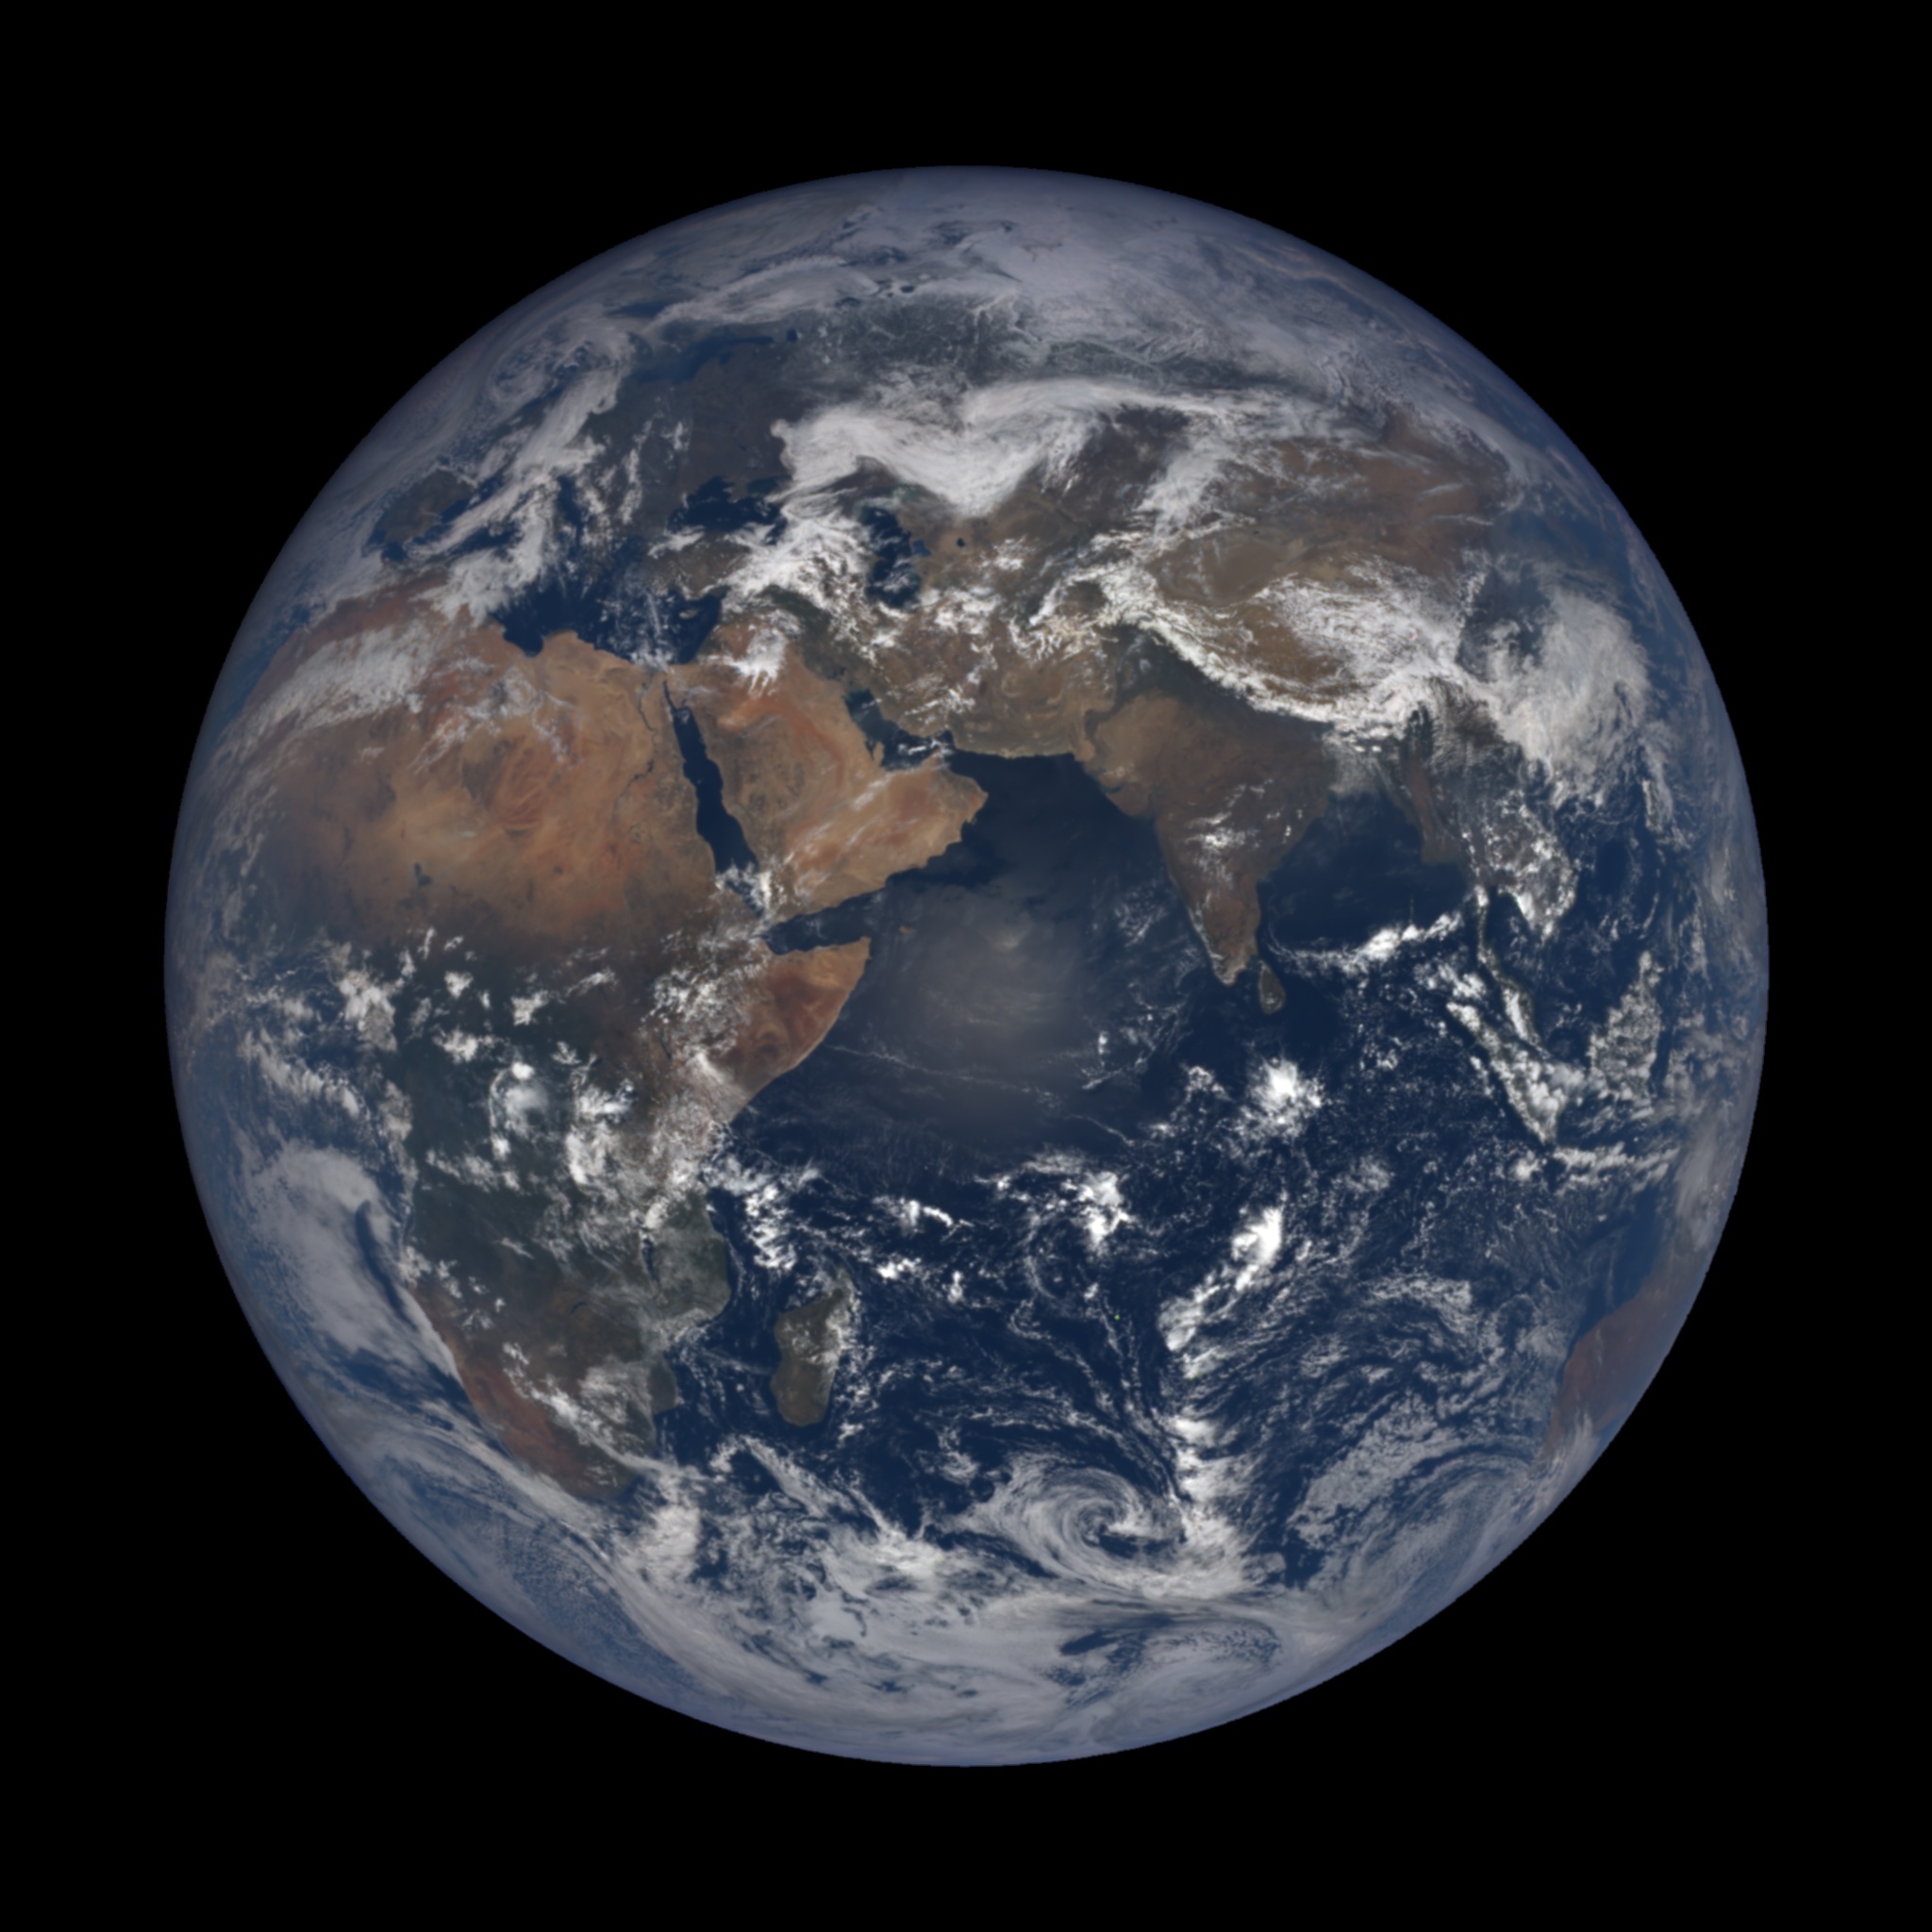
\includegraphics[width=5cm]{images/epic1}
%			\includegraphics[width=7cm]{images/fdl}
\end{columns}
\small\raggedleft(Large et al., 1954)
\end{center}

\vfill
\end{frame}
}

%\begin{frame}
%
%\frametitle{Photosynthesis}
%%	
%%	Photosynthesis
%
%\centering
%\begin{tikzpicture}
%\node(in){$6{\text{CO}}_{2}+6{\text{H}}_{2}\text{O}$};
%\node[right=of in, label={light absorbtion $\Delta \V{x}$}](arrow){$\to$};
%\node[right=of arrow]{${\text{C}}_{\text{6}}{\text{H}}_{\text{12}}{\text{O}}_{\text{6}}+{\text{6O}}_{\text{2}}$};
%\end{tikzpicture}
%%	
%%	\begin{equation*}
%%	6{\text{CO}}_{2}+6{\text{H}}_{2}\text{O}\to 
%%	\end{equation*}
%\end{frame}

\newcommand{\rastergrid}{
\begin{tikzpicture}
% each layer
\begin{scope}[scale=2]

% raster size
\def\d{0.7}		

% distance layer
\def\s{\d*5}

\foreach \i in {1,...,6}
{		
\begin{scope}[
yshift=\s*\i,every node/.append style={
yslant=0.5,xslant=-1},yslant=0.5,xslant=-1
]
%\draw[step=3.33mm] (0,0) grid (1,1);
%\fill[black,fill opacity=.9] (0.333,0.333) rectangle (0.333,0.333);    	    	  

\foreach \row in {0,...,2}{
\foreach \col in {0,...,2}{
\draw[tumblack, fill=tumblue!\pdfuniformdeviate 40,fill opacity=1,rounded corners=1] (\col*\d/3,\row*\d/3) rectangle (\col*\d/3+\d/3, \row*\d/3+\d/3);
%                 \draw[black, fill=black!\pdfuniformdeviate 40,fill opacity=1,rounded corners=1] (\col*\d/3,\row*\d/3) rectangle (\col*\d/3+\d/3, \row*\d/3+\d/3);
}
}

%\draw[step=3.33mm] (0,0) grid (1,1);
%\fill[white,fill opacity=.9] (0,0) rectangle (1,1);
\end{scope}
}
\end{scope}
\end{tikzpicture}
}


%\begin{frame}
%\frametitle{Spectral Band}
%\end{frame}


\begin{frame}
\frametitle{Multi-temporal Vegetation Modeling}

\begin{columns}
\column{.5\textwidth}

\begin{tikzpicture}
\node[] at (0,0){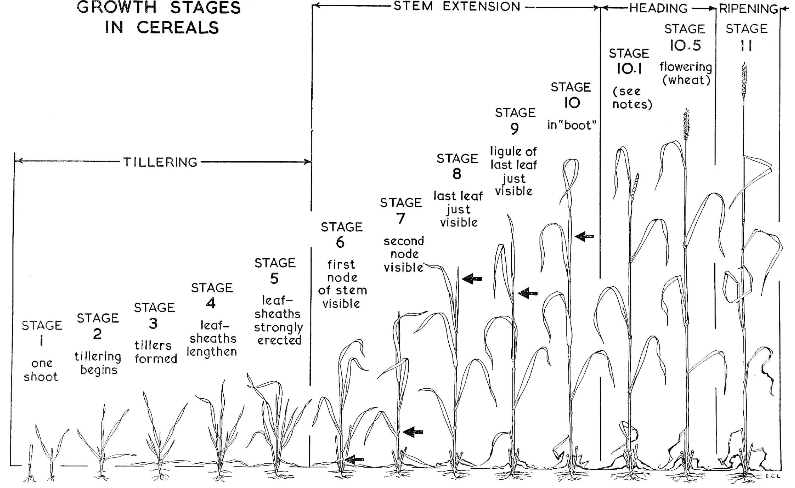
\includegraphics[width=\textwidth]{images/Large1954_cerial_growth_stages}};

%		\draw[step=1.0,black,thin, fill=none] (-2,-2) grid (2,2);

\visible<-1>{\draw [fill=white, draw=none, opacity=0.8] (-0.8,-3) rectangle (2,2.5);}
\visible<-2>{\draw [fill=white, draw=none, opacity=0.8] (2,-3) rectangle (5,2.5);}

\visible<1>{\node[rotate=190] at (-2.5,1.5){
\includegraphics[width=15mm]{images/icons/sat2}};}
\visible<2>{\node[rotate=225] at (-2.5,1.5){
\includegraphics[width=15mm]{images/icons/sat2}};}
\visible<3->{\node[rotate=260] at (-2.5,1.5){
\includegraphics[width=15mm]{images/icons/sat2}};}


\visible<4->{\node at (-1.5,1.4) {
\includegraphics[width=10mm]{images/cloud}};}

\end{tikzpicture}

\column{.5\textwidth}

{\Large
\only<1>{
\begin{equation*}
f_\text{vegetation}(\V{X}_t)
\end{equation*}
}
\only<2>{
\begin{equation*}
f_\text{vegetation}(\V{X}_t,\V{X}_{t+1})
\end{equation*}
}
\only<3>{
\begin{equation*}
f_\text{vegetation}(\V{X}_t,\V{X}_{t+1},\V{X}_{t+2})
\end{equation*}
}
}


\vspace{2em}


\visible<1->{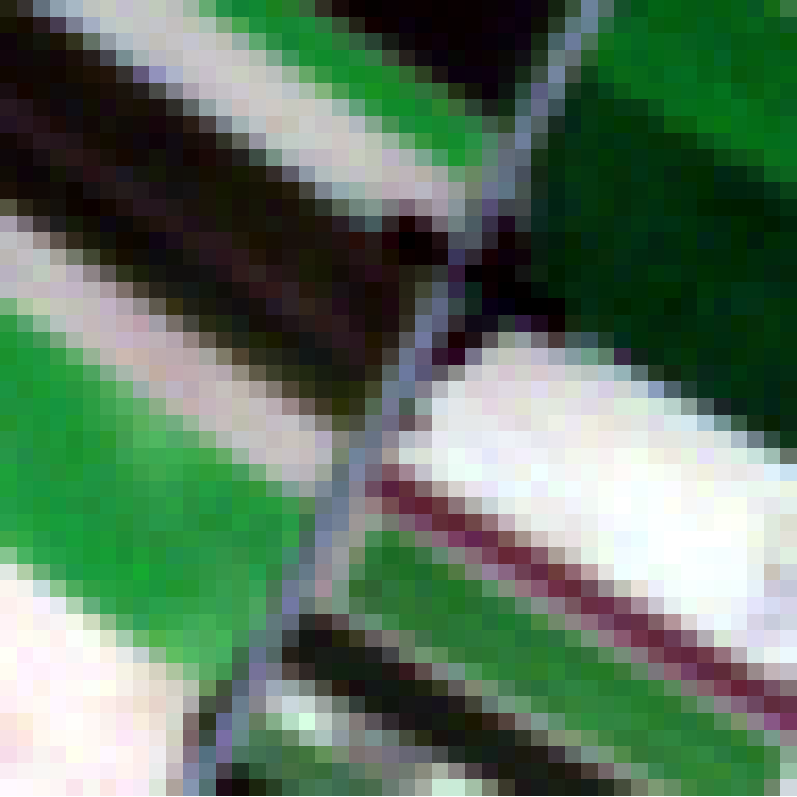
\includegraphics[width=.22\textwidth]{images/s2grid/1}}
\visible<2->{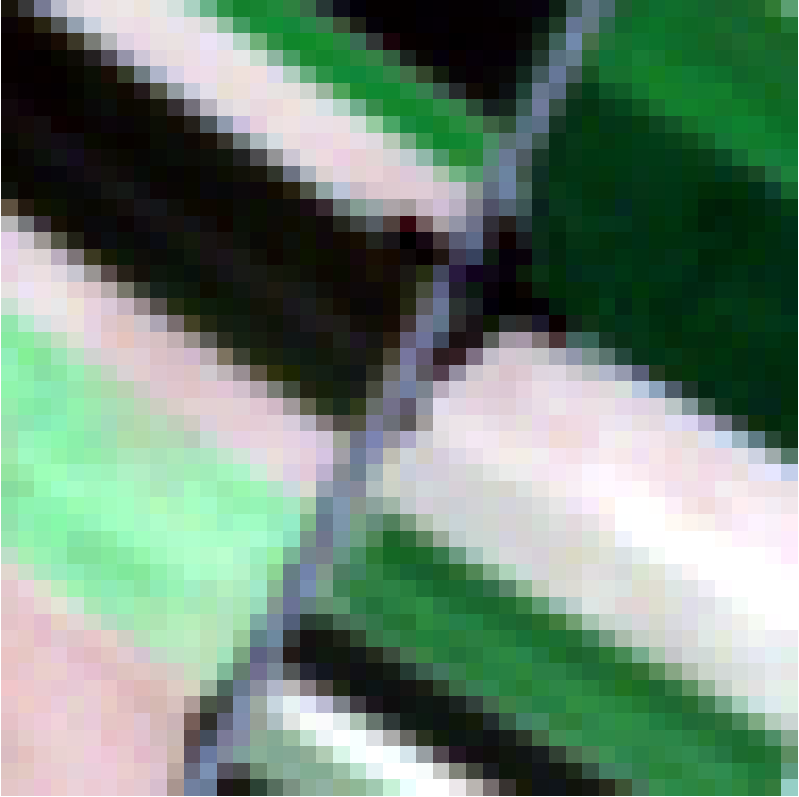
\includegraphics[width=.22\textwidth]{images/s2grid/2}}
\visible<3->{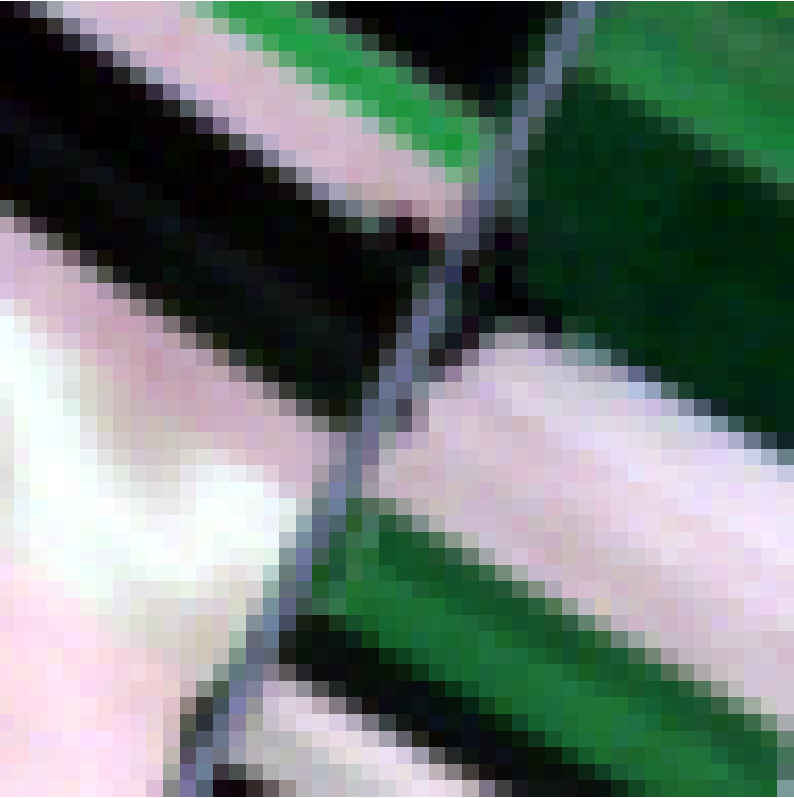
\includegraphics[width=.22\textwidth]{images/s2grid/3}}
\visible<4->{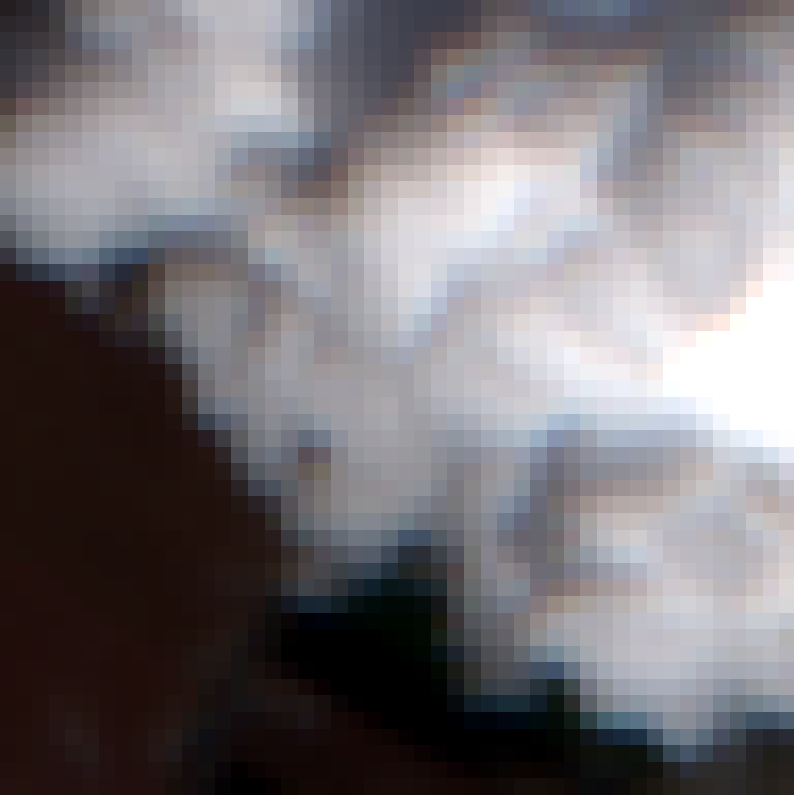
\includegraphics[width=.22\textwidth]{images/s2grid/4}}

\vspace{1em}

{\small 
Large, E. C. (1954). Growth stages in cereals illustration of the Feekes scale. Plant pathology, 3(4), 128-129.
}


\end{columns}
\end{frame}


\begin{frame}
\frametitle{Problem Definition}
\Large


\centering\begin{tikzpicture}[node distance=0em]
\visible<2->{\node(y){\V{y}};}
\visible<2->{\node[right=of y](equals){$=$};}
\node[right=of equals](f){$f_\text{vegetation}$};
\visible<1->{\node[right=of f](x){$(\V{X}_t,\V{X}_{t+1},\V{X}_{t+2})$};}

\end{tikzpicture}

\vspace{1em}
\raggedright

\begin{description}\setlength\itemsep{1em}
	\item[\color{tumblue}Problem:]<1-> \textbf{un/self-supervised learning} of a vegetation model \textbf{is difficult}
	\item[\color{tumblue}Solution:]<2-> re-framing as \textbf{supervised classification} of crop type labels
	\item[\color{tumblue}Intuition:]<3-> A \textbf{supervised classification model} must \textbf{internalize} a learned \textbf{discriminative model} for the \textbf{vegetation}
\end{description}

\end{frame}


\begin{frame}
\frametitle{Multi-temporal Earth observation}
\centering
\begin{tikzpicture}[scale=2]
%\draw[fill=tumblue, draw=none, opacity=0.5](-1,0) circle (1.5);
\node[fill=tumgraylight, draw=none, opacity=0.5, circle, minimum width=6cm, label=Earth Observation] at (-1,0){};

\node[fill=tumgraylight, draw=none, opacity=0.5, circle, minimum width=6cm, label=Machine Learning] at (1,0){};

\visible<1->{
	\node[font=\bfseries, circle, fill=tumbluelight, text width=2.5cm] (vhr) at (-1.5,.7) {high spatial \\ resolution};
	\node[font=\bfseries, circle, fill=tumorange!50, text width=2.5cm] (cv) at (1.5,.7) {computer vision methods};
	\draw[stealth-stealth, very thick] (vhr) -- node[midway,above]{well established} (cv);
}

\visible<2->{
	\node[font=\bfseries, circle, fill=tumbluelight, text width=2.5cm] (mt) at (-1.5,-.7) {high temporal resolution};
	\node[font=\bfseries, circle, fill=tumorange!50, text width=2.5cm] (nlp) at (1.5,-.7) {natural \\ language \\ processing};
	\draw[stealth-stealth, dotted] (mt) -- node[midway,above]{hardly anyone} (nlp);
}

\visible<3->{
	\node[fit=(nlp)(mt), draw, inner sep=.5em, rounded corners, thick, label=above:{\bfseries \Large my focus}]{};
}
%\draw[-stealth] (cv) -- (0,0);

%\draw[-stealth, very thick] (phd) -- (0,, fil0);
\end{tikzpicture}

\end{frame}

\begin{frame}
\frametitle{Example Analogy to Natural Language Processing}
\setrand{0}{100}{0.01}{1}
	\newcommand{\drawmatrix}{
		\left(\begin{matrix}\nextrand\thisrand\\\nextrand\thisrand\\\nextrand\thisrand\end{matrix}\right)
	}

	\newcommand{\image}[1]{
		\begin{tikzpicture}
			\node(img){\includegraphics[width=2cm]{#1}};
			\node[minimum width=.5em,minimum height=.5em, fill=tumbluelight, xshift=-1em] at (img)(rect){};
			
			\node[right=of rect, fill=tumbluelight,, inner sep=.2em, rounded corners=1em,  opacity=.2](m){$\drawmatrix$};
			\draw[tumbluelight] (rect.north) -- (m.north);
			\draw[tumbluelight] (rect.south) -- (m.south);
		\end{tikzpicture}
	}

	
	\begin{tikzpicture}[node distance=1em]
		\node[font=\scriptsize](e1){\image{images/analogy_examples/170127_snow.png}};
		\node[right=of e1, font=\scriptsize](e2){\image{images/analogy_examples/160929_clear.png}};
		\node[right=of e2, font=\scriptsize](e3){\image{images/analogy_examples/161115_cloudy.png}};
		\node[right=of e3, font=\scriptsize](e4){\image{images/analogy_examples/160728_partlycloudy.png}};
		
		\node[below=of e1, font=\scriptsize](t1){$E(\text{\textbf{The}})=\drawmatrix$};
		\node[below=of e2, font=\scriptsize](t2){$E(\text{\textbf{eagle}})=\drawmatrix$};
		\node[below=of e3, font=\scriptsize](t3){$E(\text{\textbf{has}})=\drawmatrix$};
		\node[below=of e4, font=\scriptsize](t4){$E(\text{\textbf{landed}})=\drawmatrix$};
		
		\node[above=of e1](x1){$\V{x}_1$};
		\node[above=of e2](x2){$\V{x}_2$};
		\node[above=of e3](x3){$\V{x}_3$};
		\node[above=of e4](x4){$\V{x}_4$};
		
		\node[right= 7em of e4](eo){$f(\M{X})$};
		\node[right= 7em of t4](nlp){$f(\M{X})$};
		
		\draw[-stealth] (e4) -- node[midway,above]{EO model} (eo);
		\draw[-stealth] (t4) -- node[midway,above]{NLP model} (nlp);
	\end{tikzpicture}
\end{frame}
